\setcounter{chapter}{2}
\chapter[\MakeUppercase{Kết quả mô phỏng, thực nghiệm hệ thống}]{Kết quả mô phỏng, thực nghiệm hệ thống}

Trong chương này, trình bày việc triển khai thuật toán MUSIC trên GNU Radio với dữ liệu: mô phỏng từ Matlab; giả lập BladeRF từ các khối trên GNU Radio; BladeRF thực. Từ đó rút ra so sánh, đánh giá kết quả thực tế so với mô phỏng.
%mô phỏng ảnh hưởng của: suy giảm, tạp âm, nhiễu đa đường đến độ chính xác của thuật toán cũng như kiểm tra hoạt động của việc lập trình các khối OTT trên GNU Radio. Sau đó triển khai trên các thiết bị SDR rút ra so sánh, đánh giá kết quả thực tế so với mô phỏng ban đầu.

\section{Mô phỏng hệ thống trên GNU Radio}

\subsection{Mô phỏng với dữ liệu Matlab}

Trước hết, sử dụng tín hiệu mô phỏng từ Matlab xuất ra file \textit{.mat} rồi đưa vào GNU Radio và thực hiện ước lượng hướng sóng đến từ dữ liệu, việc này đảm bảo việc lập trình khối hoạt động hiệu quả và giúp đánh giá được sai số lý tưởng của thuật toán MUSIC trước khi mô phỏng tín hiệu BladeRF. Vẫn áp dụng mô hình tín hiệu như ở mục 1.3, các thông số mô phỏng trên bảng 3.1.
%{\renewcommand\labelitemi{}
%\begin{itemize}
%          \item $f = 923\textrm{ MHz}$                \hspace{1.6cm}\% Tần số
%	\item $\lambda = c \div f = 0,325\textrm{ m}$	\hspace{0.4cm}\% Bước sóng
%	\item $M = 2$				\hspace{2.88cm}\% Số phần tử anten của mảng thu
%	\item $d = 0.5 \times \lambda$		\hspace{2.1cm}\% Khoảng cách giữa các phần tử anten mảng thu (\textbf{ULA})
%	\item $D = 1$				\hspace{2.95cm}\% Số phần tử nguồn
%	\item $angle = 85 \times (\pi \div 180)$ \% Góc tới của tín hiệu
%	\item $gain = 0$				\hspace{2.5cm}\% Hệ số khuếch đại
%	\item $SNR = 10\textrm{ dB}$			\hspace{1.5cm}\% Tỷ lệ tín hiệu tạp âm
%	\item $k = 2 \times \pi \div \lambda$	\hspace{1.56cm}\% Hệ số sóng
%	\item $K = 5000$				\hspace{2.3cm}\% Số mẫu thu thập
%\end{itemize}
\begin{table}[!h]
	\caption{Các thông số mô phỏng hệ DOA}
	\centering
	\begin{tabular}{|l|l|l|}
		\hline
		\rowcolor[HTML]{FFECEA} 
		\multicolumn{1}{|c|}{\cellcolor[HTML]{FFECEA}\textbf{Thông số}} & \multicolumn{1}{c|}{\cellcolor[HTML]{FFECEA}\textbf{Giá trị}} & \multicolumn{1}{c|}{\cellcolor[HTML]{FFECEA}\textbf{Chú thích}} \\ \hline
		$f$ & 923 Mhz & Tần số. \\ \hline
		$\lambda$ & c $\div f$ = 0,325 m & Bước sóng. \\ \hline
		M & 2 & Số phần tử anten mảng thu. \\ \hline
		d & 0,5 $\times \lambda$ & Khoảng cách giữa các phần tử anten mảng thu (ULA). \\ \hline
		D & 1 & Số phần tử nguồn. \\ \hline
		angle & 85 $\times \pi \div$ 180 & Góc tới của tín hiệu. \\ \hline
		gain & 0 & Hệ số khuếch đại. \\ \hline
		SNR & 70 dB & Tỷ lệ tín hiệu tạp âm. \\ \hline
		k & 2 $\times \pi \div \lambda$ & Hệ số sóng. \\ \hline
		K & 1024 & Số mẫu thu thập. \\ \hline
	\end{tabular}
\label{parass}
\end{table}
\begin{subequations}
\label{eq:all}
\begin{align}
\label{eq:model_a}
    \mathbf{s} &=
    \begin{bmatrix}
   	20^{\frac{SNR}{10}}\times \mathrm{randn}(1, K) + j \times \mathrm{randn}(1, K)
    \end{bmatrix}\\
\label{eq:model_b}
    \mathbf{A} &=
    \begin{bmatrix}
	10^{\frac{gain}{10}} \times \mathrm{exp}\{j \times k \times (0:M-1) \times d \times \cos(angle)\}
    \end{bmatrix}^T \\
\label{eq:model_c}
 \mathbf{n} &=
    \begin{bmatrix}
	\mathrm{randn}(M, K) + j \times \mathrm{randn}(M, K)
    \end{bmatrix} \\
\label{eq:model_d}
 \mathbf{x} &=
    \begin{bmatrix}
	\mathbf{A}\mathbf{s} + \mathbf{n}
    \end{bmatrix}
%\end{equation} 
\end{align}
\end{subequations}

Sử dụng Matlab tạo mô phỏng dữ liệu đầu vào với những thông số như trên, thu được được ma trận $\mathbf{x}(t) \in \mathbb{C}^{2 \times 5000}$, lưu trữ vào file \textit{source.mat} bằng hàm có sẵn của Matlab. Việc tiếp theo là đưa dữ liệu mô phỏng vào GNU Radio thông qua việc tạo một khối nguồn cho file \textit{source.mat}. Đối với mục đích này, Synchronous Blocks được sử dụng: một khối loại bỏ đầu vào và thay thế bằng file dữ liệu mô phỏng từ Matlab tạo thành khối nguồn; một khối loại bỏ đầu ra tạo thành khối đích để tính toán và hiển thị giao diện DOA. Sử dụng Pỵthon để tiết kiệm thời gian viết khối, sơ đồ khối của việc mô phỏng thực hiện như hình \ref{fig:simulation}.
\begin{figure} [h]
	\centering
	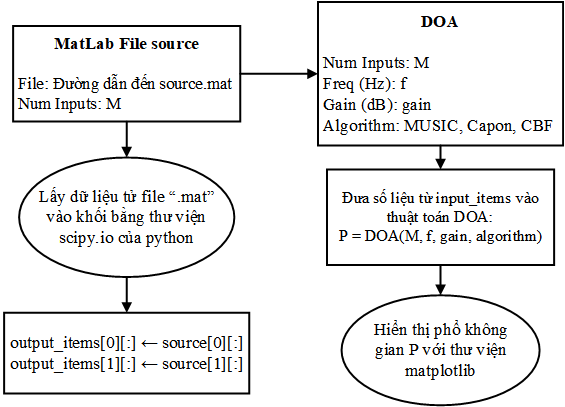
\includegraphics[width=0.8\linewidth]{figures/simulation.png}
	\caption{Sơ đồ làm việc DOA với dữ liệu mô phỏng Matlab}
	\label{fig:simulation}
\end{figure}

Liên kết hai khối với nhau và nhập các thông số đầu vào của hệ và chạy hệ thống. Kết quả trên GNU Radio Companion thu được như phụ lục hình \ref{fig:simulation1}. Tiến hành thay đổi góc đầu vào từ file dữ liệu Matlab và chạy hệ thống nhiều lần, mỗi lần sẽ thu được kết quả như hình \ref{fig:simulation2}.
\begin{figure}[!h]
%\hfill
\subfigure[Kết quả của GNU Radio]{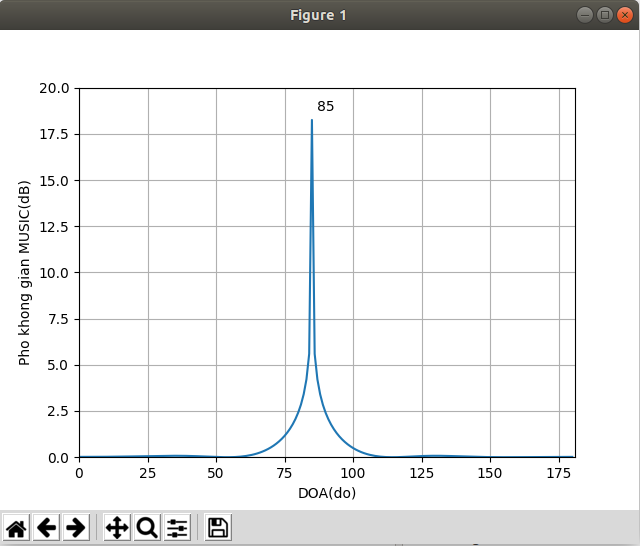
\includegraphics[width=0.49\linewidth]{figures/simulation3.png}}
\hfill
\subfigure[Kết quả của Matlab]{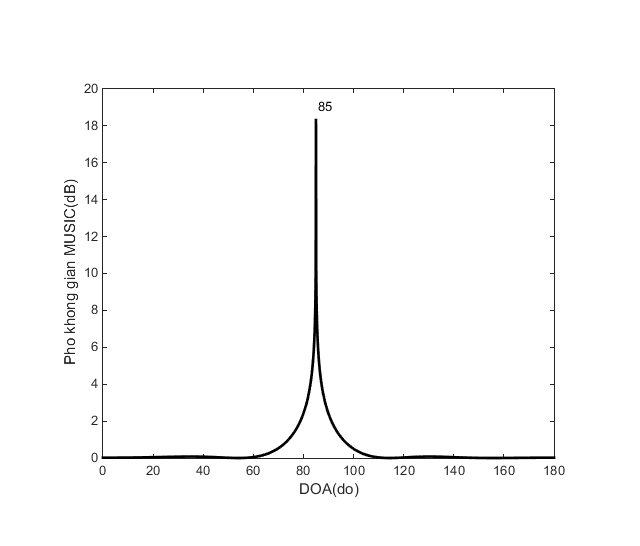
\includegraphics[width=0.49\linewidth]{figures/simulation4.png}}
\hfill
\caption{Kết quả ước lượng DOA với dữ liệu mô phỏng Matlab}
\label{fig:simulation2}
\end{figure}

Do dữ liệu mô phỏng là hoàn toàn khớp với các điều kiện lý tưởng, sai số của thuật toán MUSIC trên GNU Radio giống như trên lý thuyết \cite{Transactions1989, Quynh2015}, sử dụng thông số CRB (Cramér–Rao bound) cho một nguồn để đánh giá sai số ước lượng:
\begin{equation}
	\mathrm{CRB}(\phi) = \mathbf{J}^{-1} 
\end{equation}
với $\mathbf{J}^{-1}$ là ma trận Fisher, được biểu diễn ở phương trình (3.2):
\begin{equation}
\begin{split}
\mathbf{J} &= K \cdot \mathrm{trace} \left \{ \mathbf{R}_\mathbf{x}^{-1} \frac{\partial \mathbf{R}_\mathbf{x}}{\partial \phi} \mathbf{R}_\mathbf{x}^{-1} \frac{\partial \mathbf{R}_\mathbf{x}}{\partial \phi} \right \} \\
&= \frac{2 \mathrm{SNR}^2}{(1 + \mathrm{SNR} |\mathbf{a}|^2)^2} [2(\Re  (\mathbf{a}^{H} \dot{\mathbf{a}}))^2 + (1 + \mathrm{SNR} |\mathbf{a}|^2)(|\mathbf{a}|^2 |\dot{\mathbf{a}}|^2 - |\mathbf{a}^H \dot{\mathbf{a}}|^2)]
\end{split} 
\end{equation}
với $\dot{\mathbf{a}}_\phi = \partial\mathbf{a}/\partial\phi$. Hình \ref{fig:RMSE} biểu diễn CRB của mảng ULA với các tham số: $M$ = 2, SNR = 70 dB, số mẫu $K$ = 1024. Như vậy, thấy rằng mảng ULA có lỗi ước lượng nhỏ với các góc ở trục vuông và sai số lớn với các góc ở trục dọc so với mảng anten thu.
\begin{figure} [!h]
	\centering
	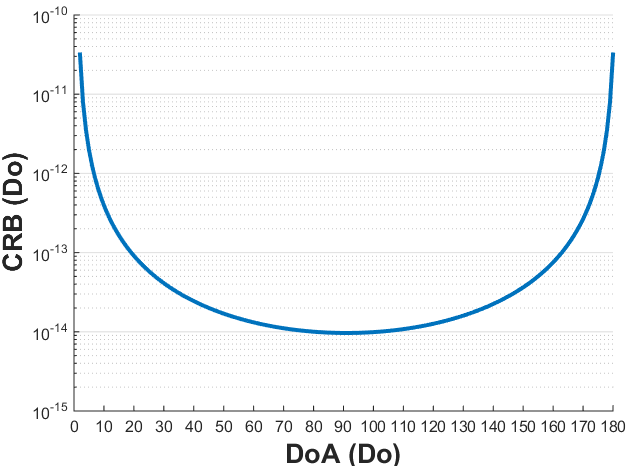
\includegraphics[width=0.64\linewidth]{figures/CRB.png}
	\caption{CRB của mảng anten ULA}
	\label{fig:RMSE}
\end{figure}

\subsection{Mô phỏng với dữ liệu giả lập BladeRF}

Sau khi đã mô phỏng thành công với dữ liệu từ Matlab, tiếp tục mô phỏng dữ liệu BladeRF thực với tín hiệu đầu vào là âm thanh được điều chế NBFM (chi tiết tham số điều chế, phổ, SNR được trình bày ở mục 3.2.1). Vẫn sử dụng thông số mô phỏng như bảng 3.1, sau khi được mã hóa, chia tín hiệu thành 2 luồng đi qua kênh truyền với các thông số như bảng \ref{tab:simu}, các khối mô phỏng tương ứng trên GNU Radio được biểu diễn ở phụ lục hình \ref{fig:bladesimu}.
\begin{table}[!h]
\centering
\caption{Các thông số mô phỏng tín hiệu BladeRF qua kênh truyền}
\arrayrulecolor{black}
\begin{tabular}{|l|l|l|} 
	\hline
	\rowcolor[rgb]{1,0.91,0.906} \multicolumn{1}{|c|}{ \textbf{Mô phỏng} } & \multicolumn{1}{c|}{\textbf{Thông số mô phỏng} } & \multicolumn{1}{c|}{\textbf{Giá trị} }  \\ 
	\hline
	{\cellcolor[rgb]{0.937,0.937,0.937}}                                   & Giá trị tạp âm                                   & 0,01 (1\% biên độ tối đa của tín hiệu)  \\ 
	\hhline{|>{\arrayrulecolor[rgb]{0.937,0.937,0.937}}->{\arrayrulecolor{black}}--|}
	{\cellcolor[rgb]{0.937,0.937,0.937}}                                   & Gieo hạt của tạm âm                              & 1000                                    \\ 
	\hhline{|>{\arrayrulecolor[rgb]{0.937,0.937,0.937}}->{\arrayrulecolor{black}}--|}
	{\cellcolor[rgb]{0.937,0.937,0.937}}                                   & Số tín hiệu đa đường                             & 8                                       \\ 
	\hhline{|>{\arrayrulecolor[rgb]{0.937,0.937,0.937}}->{\arrayrulecolor{black}}--|}
	{\cellcolor[rgb]{0.937,0.937,0.937}}                                   & Phân bố nhiễu đa đường                           & Rayleigh                                \\ 
	\hhline{|>{\arrayrulecolor[rgb]{0.937,0.937,0.937}}->{\arrayrulecolor{black}}--|}
	\multirow{-5}{*}{{\cellcolor[rgb]{0.937,0.937,0.937}}Kênh truyền}      & Gieo hạt nhiễu đa đường                          & 1000                                    \\ 
	\hline
	{\cellcolor[rgb]{1,0.988,0.62}}                                        & Trễ mẫu                                          & 1000 (mẫu)                              \\ 
	\hhline{|>{\arrayrulecolor[rgb]{1,0.988,0.62}}->{\arrayrulecolor{black}}--|}
	\multirow{-2}{*}{{\cellcolor[rgb]{1,0.988,0.62}}Phần cứng BladeRF}     & Độ lệch pha ban đầu                              & 45$^{\circ}$ = 0,78539 (rad)            \\
	\hline
\end{tabular}
\label{tab:simu}
\end{table}

Chạy mô phỏng với các tệp âm thanh khác nhau, mỗi tệp chạy 5 lần và ghi lại kết quả thông số đồng bộ và vector giá trị riêng từ hệ DOA, sau đó tính trung bình và đưa vào bảng \ref{tab:kqsync}.
%Qua 2 giá trị độ trễ mẫu và độ trễ pha mà hệ tính toán được, so sánh với thông số mô phỏng đầu vào trên bảng \ref{tab:simu}, nhận thấy tín hiệu DVB-T cho kết quả khớp hoàn toàn. Với NBFM việc xác định độ trễ mẫu sai kéo theo độ lệch pha ban đầu cũng sai khác so với mô phỏng. Qua vector giá trị riêng $\textbf{E}_\textbf{s}$ của ma trận hiệp phương sai $\textbf{R}_\textbf{x}$, nhận thấy thuật toán phân biệt rõ nguồn tín hiệu và tạp âm với mức chênh lệch $10^7$ của DVB-T so với $10^2$ của NBFM.

\begin{table}[!h]
\centering
\caption{Kết quả mô phỏng đồng bộ}
\begin{tabular}{|l|c|c|cc|} 
	\hline
	\rowcolor[rgb]{1,0.91,0.906} \multicolumn{1}{|c|}{ \textbf{Nguồn tín hiệu} }                   & \textbf{Độ trễ (mẫu)}  & \textbf{Độ lệch pha (rad)}  & \multicolumn{2}{c|}{\textbf{Vector giá trị riêng} }  \\ 
	\hline
	\multirow{2}{*}{Tệp âm thanh 1}                                                                & \multirow{2}{*}{994,6}   & \multirow{2}{*}{0,72986}    & 0,00048259 & 0                                       \\
	&                        &                             & 0          & 0,04719653                              \\ 
	\hline
	\multirow{2}{*}{Tệp âm thanh 2 }                                                               & \multirow{2}{*}{991,25}  & \multirow{2}{*}{0,72999}    & 2,03512e-5 & 0                                       \\
	&                        &                             & 0          & 0,0863451                               \\ 
	\hline
	\multirow{2}{*}{\begin{tabular}[c]{@{}l@{}}Tệp âm thanh 1 bỏ\\qua trễ phần cứng \end{tabular}} & \multirow{2}{*}{}      & \multirow{2}{*}{}           & 1,241364-5 & 0                                       \\
	&                        &                             & 0          & 0,0034562                               \\
	\hline
\end{tabular}
\label{tab:kqsync}
\end{table}

Từ bảng \ref{tab:kqsync}, nhận thấy việc ước lượng độ trễ bằng tương quan chéo của tín hiệu NBFM cho kết quả chưa hoàn toàn chính xác (< 10 mẫu), kéo theo đó sẽ là sai số khi ước lượng độ lệch pha ở mức 0,056 (rad). Thông số đánh giá còn lại là ma trận vector giá trị riêng, biểu hiện sự phân biệt giữa tín hiệu và tạp âm, với tỷ lệ trung bình $10^2$ đến $10^3$, tín hiệu NBFM đủ để xuất hiện đỉnh phổ trên phổ không gian MUSIC.

Từ kết quả mô phỏng đồng bộ chưa hoàn toàn chính xác khi sử dụng NBFM, cần phải mô phỏng ước lượng hướng sóng đến dựa trên những kết quả đồng bộ phía trên để có đánh giá chính xác nhất. Kết quả sẽ được tính lỗi căn trung bình bình phương RMSE của góc thu được ($\phi$) so với góc mô phỏng ($\bar{\phi}$) như trên công thức (3.3) với D là số lần thu thập kết quả, sai số được biểu diễn trên hình \ref{fig:kqnbfm}.
\begin{equation}
	\mathrm{RMSE} = \sqrt{\frac{1}{D}\sum_{i=1}^{D}(\phi_i - \bar{\phi}_i)} 
\end{equation}

\begin{figure} [!ht]
	\centering
	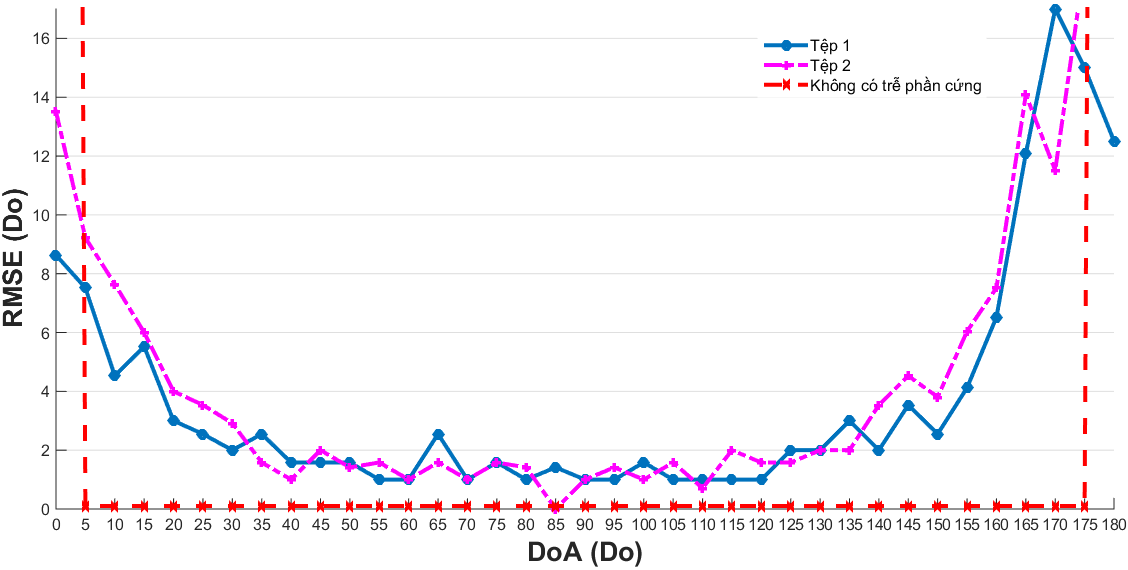
\includegraphics[width=1\linewidth]{figures/kqnbfm.png}
	\caption{RMSE: Mô phỏng dữ liệu BladeRF qua kênh truyền}
	\label{fig:kqnbfm}
\end{figure}

Như vậy so với CRB hay mô phỏng hệ thống không chịu ảnh hưởng bởi trễ phần cứng gây ra bởi BladeRF thì dạng đồ thị của RMSE khi sử dụng NBFM làm tín hiệu nguồn phát vẫn giữ được đúng hình dạng là sai số nhỏ ở những góc gần 90$^{\circ}$ và tăng dần ở hai biên phổ không gian. Tuy nhiên với các tệp âm thanh nguồn khác nhau, việc đồng bộ hệ BladeRF sẽ cho kết quả khác nhau và dẫn đến sai số góc ước lượng cũng là khác nhau nhưng không quá nhiều.

Kết luận lại, dù vẫn còn sai số trong việc đồng bộ hệ BladeRF tuy nhiên sai số vẫn đủ nhỏ để tiếp tục sử dụng tín hiệu NBFM thực hiện hệ DOA trên hệ thống BladeRF thực.

\section{Thực nghiệm hệ thống}

Với tiền đề là việc mô phỏng thành công  được dữ liệu BladeRF trên GNU Radio, tiếp theo là thực nghiệm hệ thống DOA trên hệ BladeRF thực, trong phần này sẽ trình bày điều kiện và kết quả thực nghiệm, cuối cùng đưa ra nhận xét từ kết quả thu được.

\subsection{Tín hiệu nguồn phát và thiết lập hệ thu}

Dữ liệu thực tế được dùng cho hệ tìm hướng sóng đến rất da dạng như: tín hiệu FM của các đài phát thanh, tín hiệu chuẩn DVB-T của đài truyền hình, GSM hay WiFi,... Trong khóa luận này, tín hiệu NBFM được lựa chọn để làm tín hiệu nguồn phát, vừa để đồng bộ hệ SDR thu, vừa để làm tín hiệu nguồn cho việc xác định hướng sóng đến. Lý do lựa chọn NBFM, vì đây là điều chế tín hiệu băng hẹp phù hợp với mô hình tín hiệu ban đầu của thuật toán.

NBFM: Điều chế NBFM trên GNU Radio với file nguồn là file âm thanh nén ở chuẩn WAV (Waveform Audio File Format). Flow-graph phụ lục hình \ref{fig:NBFM} là sơ đồ điều chế tiêu chuẩn NBFM cho tệp âm thanh WAV, với tín hiệu đầu ra băng hẹp 5,3 kHz (có phổ như hình \ref{fig:nbfmspectrum}, SNR trên 70 dB) và chỉ cần một bộ lọc thông thấp 5 kHz và khối giải điều chế NBFM tiêu chuẩn là đủ để giải điều chế.
\begin{figure} [!h]
	\centering
	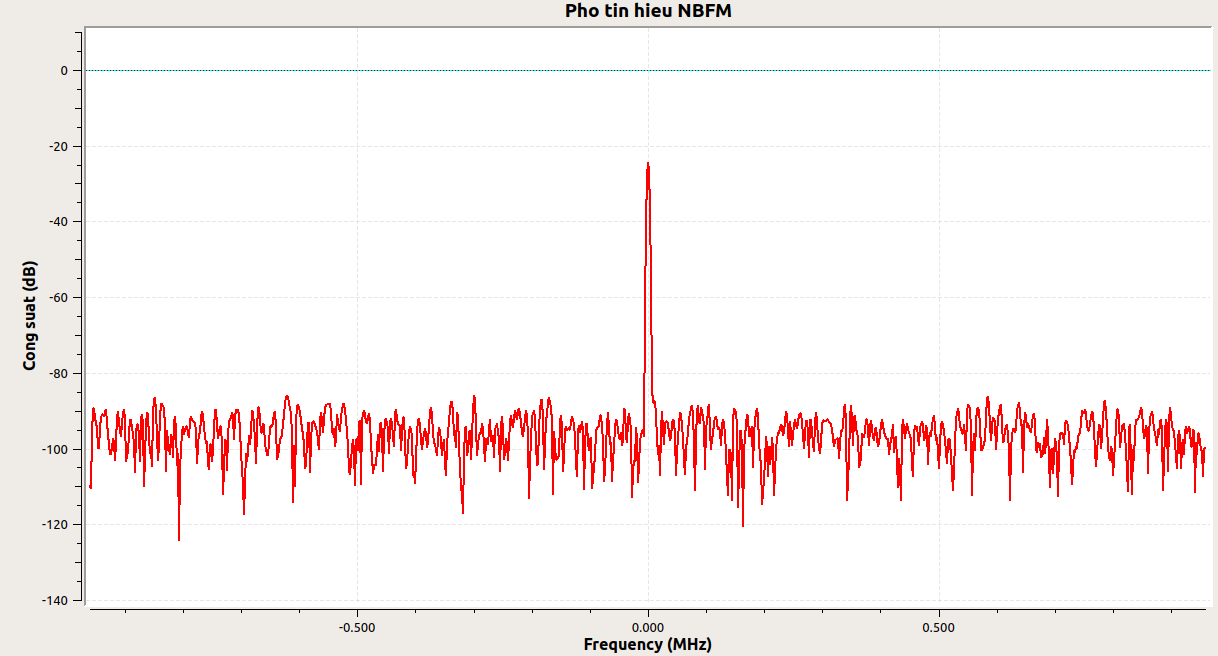
\includegraphics[width=1\linewidth]{figures/nbfmspectrum.png}
	\caption{Phổ của tín hiệu tín hiệu NBFM}
	\label{fig:nbfmspectrum}
\end{figure}

%DVB-T: Điều chế chuẩn DVB-T trên GNU Radio với file nguồn là file video nén ở chuẩn TS (Transport Stream). Flow-graph \ref{fig:dvbt} truyền video ở băng thông 8 MHz, chòm sao QPSK, tốc độ mã 7/8, khoảng bảo vệ 1/32, tốc độ lấy mẫu 10 MHz, tần số 923 MHz. Chi tiết hơn về việc sử dụng BladeRF truyền nhận DVB-T có tại \cite{BogdanDIA2015}.
%\begin{figure} [!h]
%	\centering
%	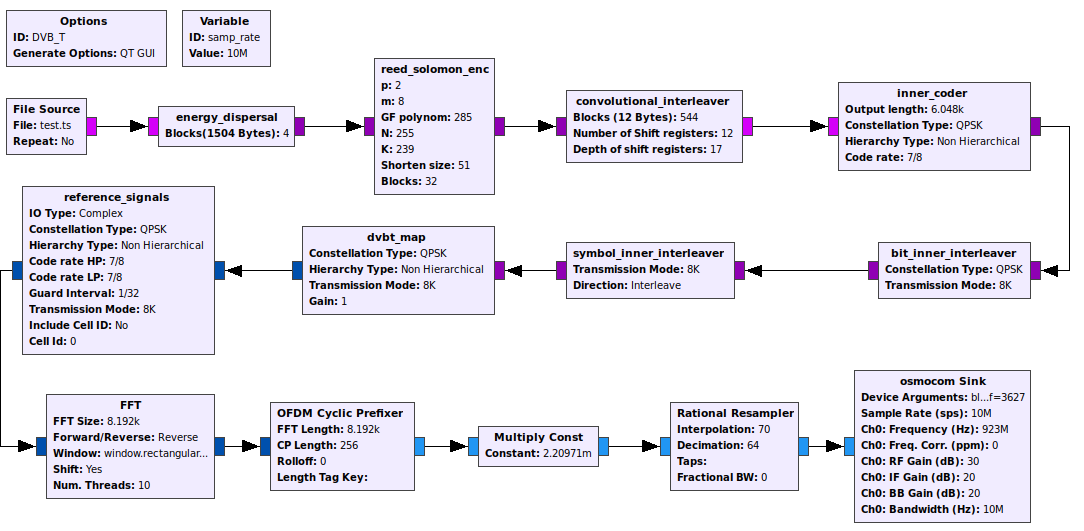
\includegraphics[width=0.95\linewidth]{figures/dvbt.png}
%	\caption{Flow-graph truyền tín hiệu DVB-T}
%	\label{fig:dvbt}
%\end{figure}

Đối với hệ thu, các bước đồng bộ và ước lượng DOA trình bày ở Chương 2 được kết hợp với nhau trên GNU Radio. Trước hết thực hiện các thiết lập trên \textit{bladeRF-cli} như chia sẻ xung đồng hồ qua cổng SMB, hiệu chỉnh CFO của BladeRF. Sau đó sử dụng flow-graph trên phụ lục hình \ref{fig:DoA_FM} phía dưới để đồng bộ và ước lượng DOA. 
%\newpage

\subsection{Tình huống thực nghiệm}

Bố trí hệ thu phát sử dụng BladeRF để triển khai việc ước lượng hướng sóng đến, trên hình \ref{fig:realsys} là hệ thống được cài đặt hoàn chỉnh, gồm 1 BladeRF phát và 2 BladeRF thu, cả 3 anten được sử dụng đều là anten không định hướng VERT2450. Cấu hình phần cứng và phần mềm của 2 máy tính thực hiện việc phát và thu trong khóa luận được nêu ra trong bảng \ref{table:hw}. Tần số được chọn là 923 MHz, là tần số nằm trong khoảng giữa của đường lên và xuống trong GSM900.
\begin{figure} [!h]
	\centering
	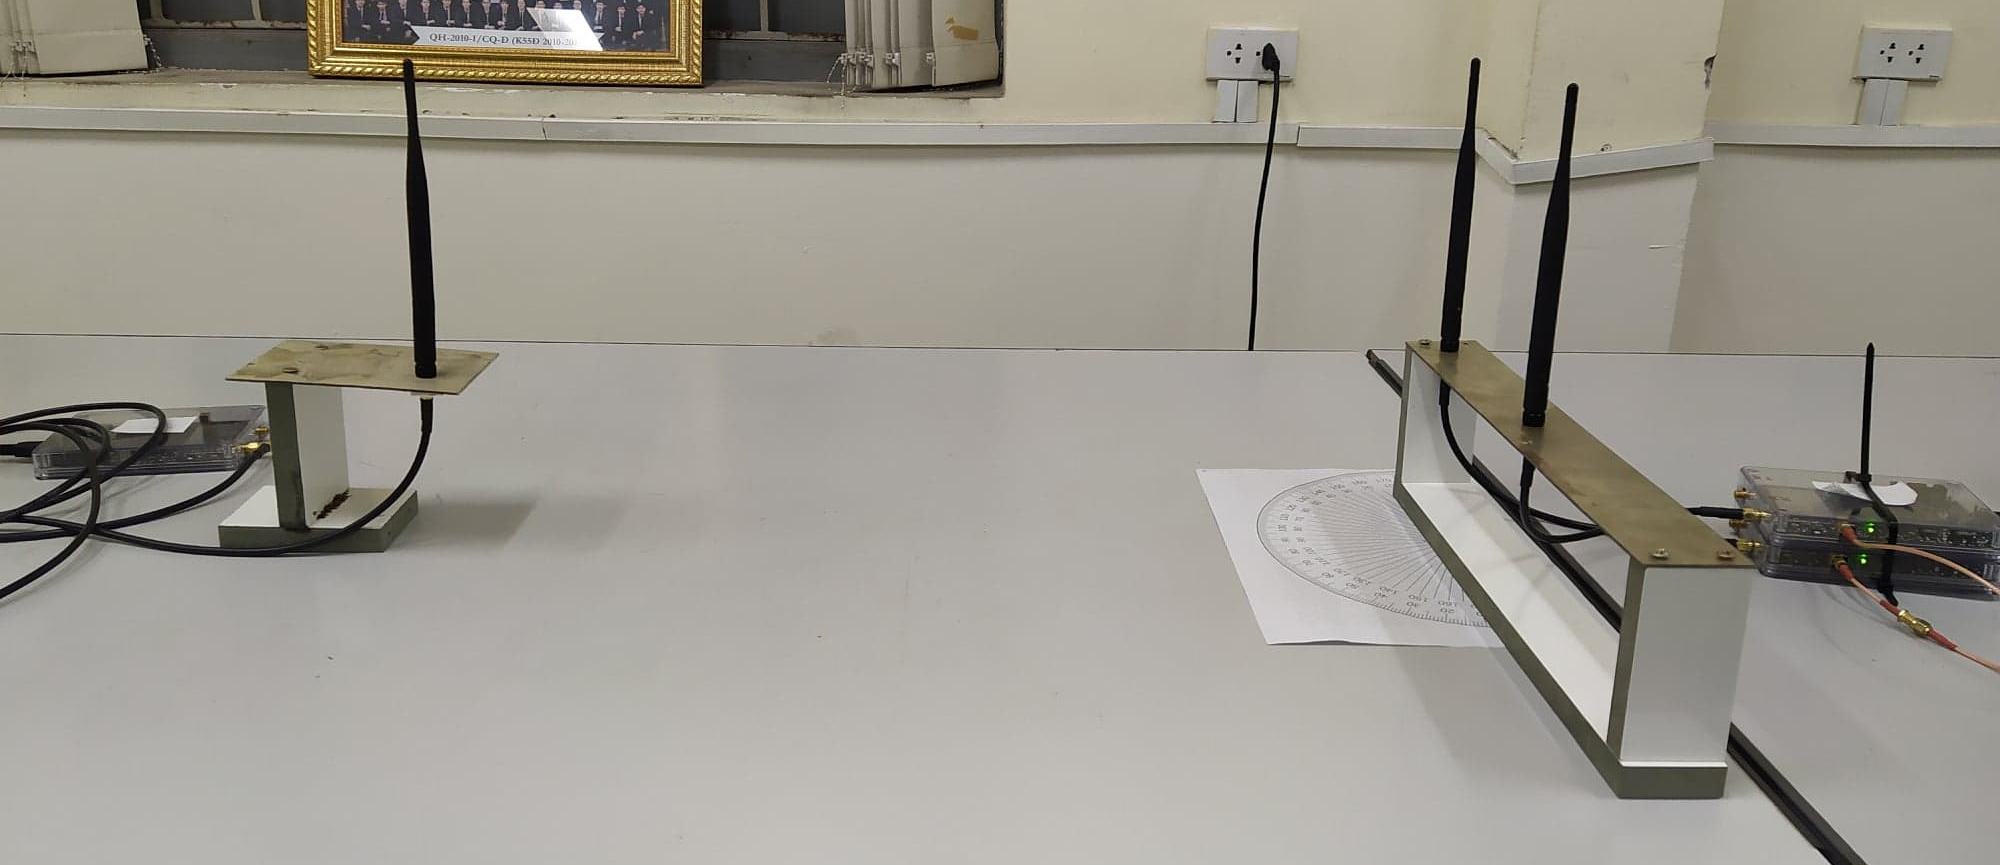
\includegraphics[width=1\linewidth]{figures/realsys.jpg}
	\caption{Sơ đồ bố trí hệ DOA thực}
	\label{fig:realsys}
\end{figure}
\begin{table}[!h]
\centering
\caption{Thông số máy tính}
\begin{tabular}{|l|c|c|} 
	\hline
	\rowcolor[rgb]{1,0.91,0.906} \multicolumn{1}{|c|}{ \textbf{Thông số} } & \textbf{Bên phát}    & \textbf{Bên thu}     \\ 
	\hline
	CPU                                                                    & Intel Core I5-4800MQ & Intel Core I5-4210M  \\ 
	\hline
	RAM                                                                    & 8 GB                 & 8 GB                 \\ 
	\hline
	Hệ điều hành                                                           & Ubuntu 16.04 LTS     & Ubuntu 18.04 LTS     \\ 
	\hline
	Phiên bản GNU Radio                                                    & 3.7.11               & 3.7.11               \\
	\hline
\end{tabular}
\label{table:hw}
\end{table}

Điều kiện thực nghiệm là phòng 204, nhà G2, Đại học Công Nghệ - Đại học Quốc Gia Hà Nội, tiến hành thực nghiệm 350 lần, xác định hướng sóng đến từ các góc khác nhau, để giảm thiểu sai số chủ quan độ phân giải khi thực nghiệm ở mức 5$^{\circ}$, bố trí hệ thống ở 3 vị trí khác nhau để đưa ra ảnh hưởng của môi trường đến độ chính xác của hệ DOA.
\newpage
\subsection{Kết quả thực nghiệm}

\begin{itemize}
	\item[$\ast$] \textbf{Phổ không gian}
\end{itemize} 

Hình \ref{fig:kqsync} biểu diễn kết phổ không gian của thuật toán MUSIC trên GNU Radio trong trường hợp: có tín hiệu đến ở góc 90$^{\circ}$, không có tín hiệu nào đến và tín hiệu mô phỏng từ Matlab.

\begin{figure} [!h]
	\centering
	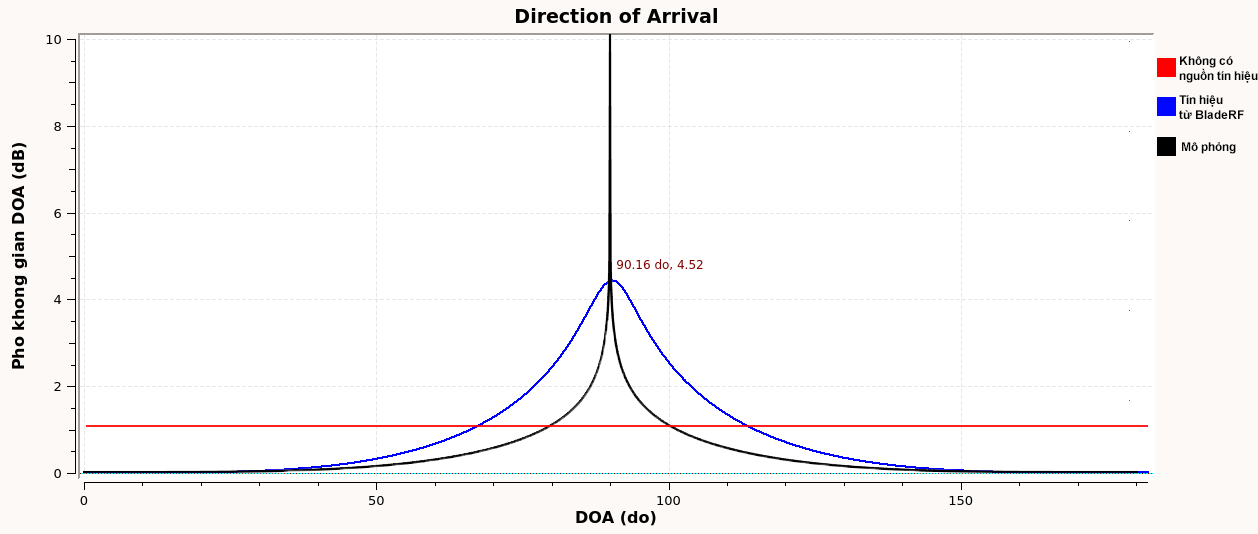
\includegraphics[width=1\linewidth]{figures/kqsync.png}
	\caption{So sánh phổ không gian trên thực tế và mô phỏng}
	\label{fig:kqsync}
\end{figure}

Hình dạng phổ không gian khi thực nghiệm là giống với kết quả khi mô phỏng, tuy nhiên về đỉnh phổ thì lại thấp hơn so với mô phỏng và độ rộng của đỉnh phổ cũng lớn hơn mô phỏng, điều này xảy ra do tín hiệu thực có biên độ chênh lệch với nhau lớn, đây là vấn đề do phần cứng, hệ số khuếch đại, việc khắc phục sẽ được thực hiện trong tương lai. Còn khi không có tín hiệu đến, phổ DOA đã cho kết quả đúng khi không xuất hiện đỉnh phổ nào.

\begin{itemize}
	\item[$\ast$] \textbf{Kết quả đồng bộ}
\end{itemize} 

Kết quả mô phỏng khi hệ thống DOA đồng bộ và không đồng bộ như hình \ref{fig:simukq}, kết cho cho thấy sau khi được đồng bộ về lượng mẫu trễ và pha sai lệch giữa các tín hiệu từ BladeRF, kết quả phổ DOA thu được sẽ giữ ở một đỉnh phổ ổn định và chính xác, còn khi hệ BladeRF chưa đồng bộ đỉnh phổ liên tục nhảy giữa các vị trí khác nhau, không thể xác định hướng sóng đến.

\begin{figure} [!h]
	\centering
	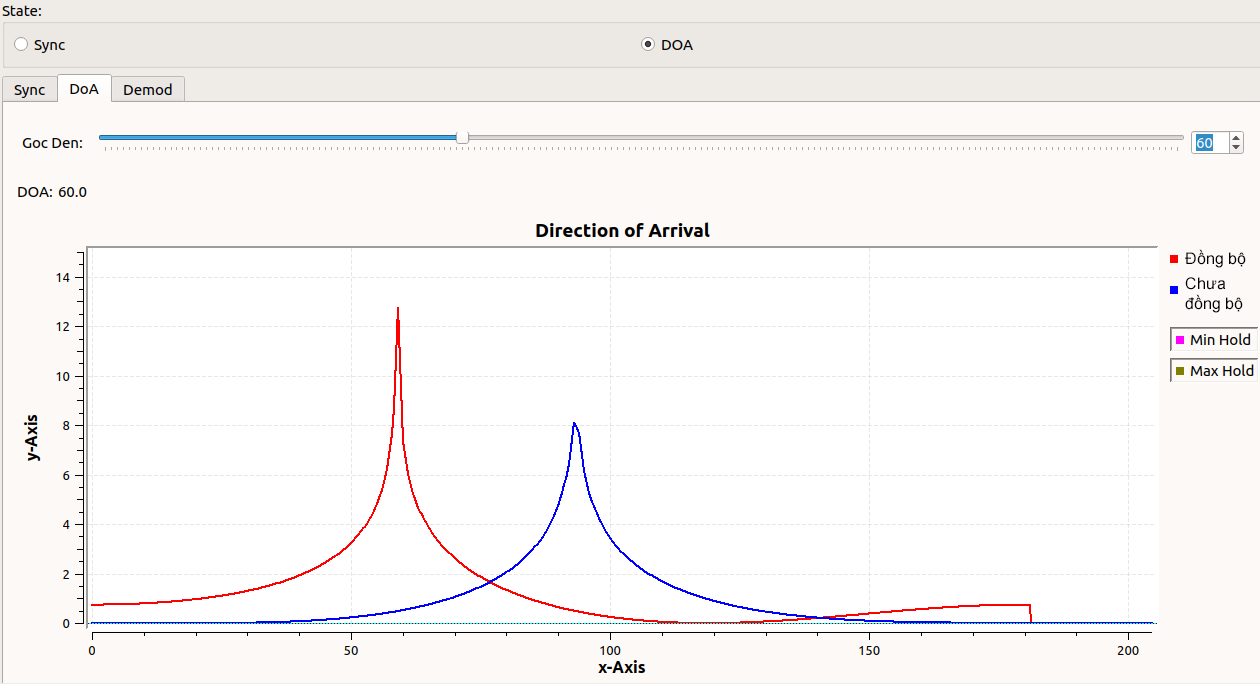
\includegraphics[width=1\linewidth]{figures/simukq.png}
	\caption{Kết quả DOA mô phỏng khi hệ SDR đồng bộ}
	\label{fig:simukq}
\end{figure}
\newpage
Qua kiểm nghiệm thực tế, kết quả cũng thu được như trên mô phỏng tuy nhiên độ rộng của đỉnh phổ thì lớn hơn mô phỏng nhưng kết quả ước lượng vẫn chính xác khi hệ BladeRF được đồng bộ. Đối với hệ BladeRF chưa được đồng bộ, góc ước lượng được luôn thay đổi và không thể xác định hướng sóng đến.

\begin{figure} [!h]
	\centering
	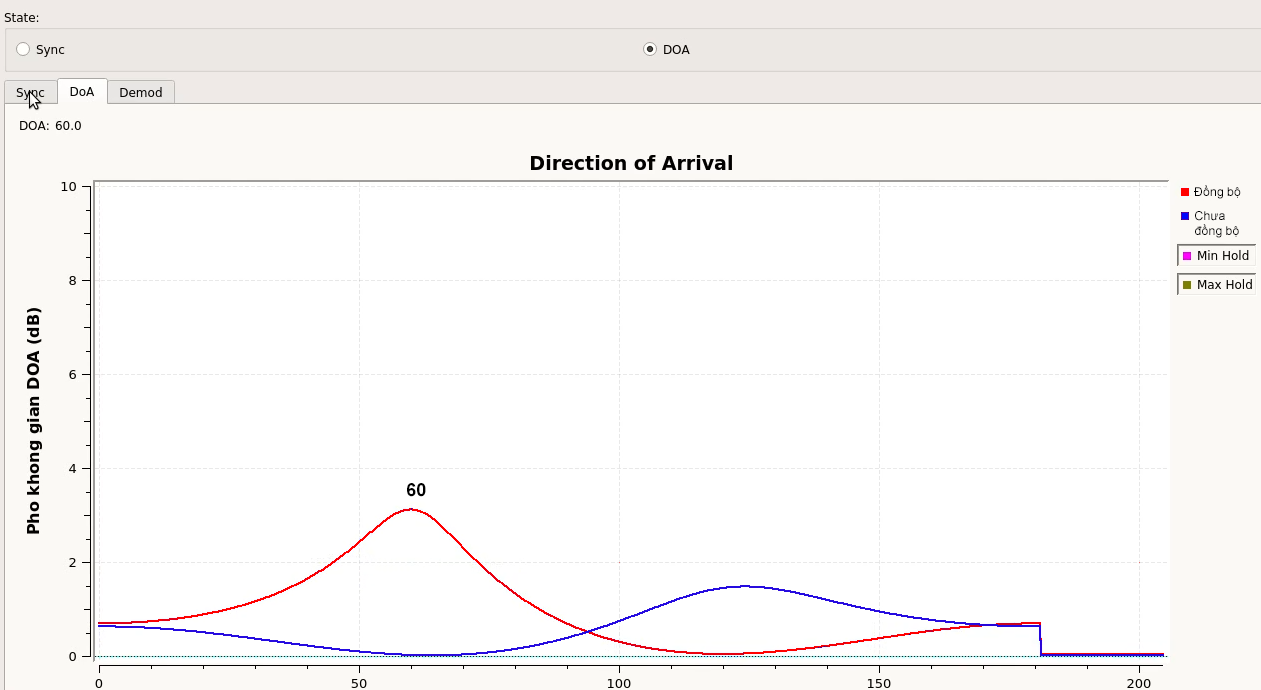
\includegraphics[width=1\linewidth]{figures/kqreal.png}
	\caption{Kết quả DOA thực nghiệm khi hệ SDR đồng bộ}
	\label{fig:kqreal}
\end{figure}
\newpage
\begin{itemize}
	\item[$\ast$] \textbf{Khảo sát lỗi ước lượng của hệ thống}
\end{itemize} 

\textbf{- Kết quả ước lượng theo độ $\phi = 0 \rightarrow 180$}

Hình \ref{fig:kq1} là RMSE của quá trình thực nghiệm ước lượng DOA trên BladeRF thực so với kết quả mô phỏng dữ liệu BladeRF. Nhận thấy, dạng biểu đồ RMSE thu được từ thực nghiệm là tương đồng với mô phỏng và CRB được ước lượng ở hình \ref{fig:RMSE}, sai số ở các góc gần 90$^{\circ}$ nhỏ, và tăng dần ở các góc ở hai biên của phổ không gian.

Ở khoảng góc từ 60$^{\circ}$ đến 135$^{\circ}$, sai số dưới 6$^{\circ}$, và do chỉ sử dụng 2 phần tử anten mảng thu nên mức sai số này là chấp nhận được.
\begin{figure} [!h]
	\centering
	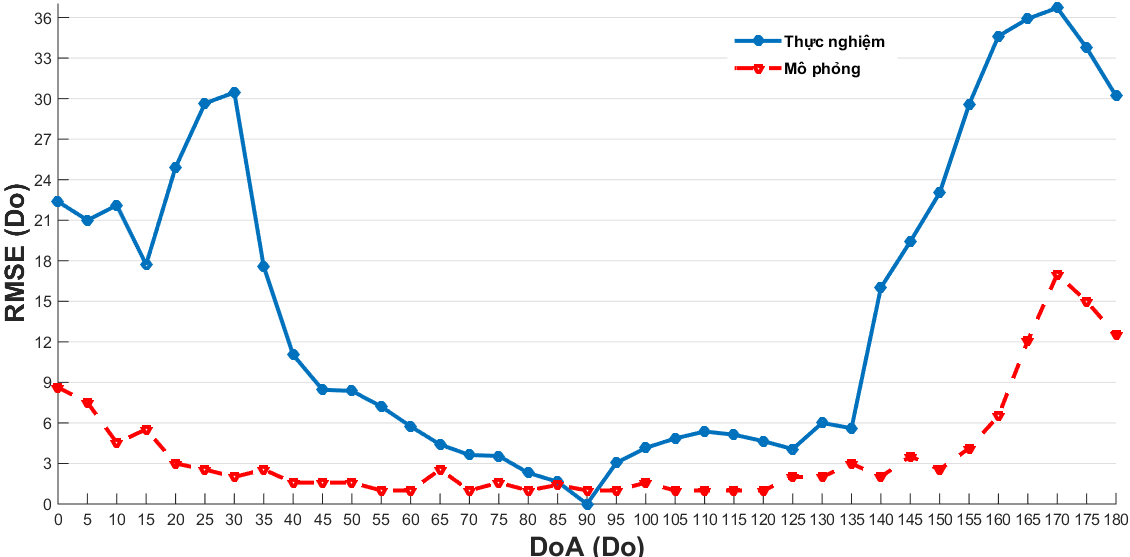
\includegraphics[width=1\linewidth]{figures/kq1.png}
	\caption{RMSE: DOA thực nghiệm và mô phỏng}
	\label{fig:kq1}
\end{figure}

\textbf{- Kết quả ước lượng theo vị trí}

Thực nghiệm thêm để xem xét vị trí đặt hệ DOA hay kênh truyền có ảnh hưởng đến kết quả ước lượng hướng sóng đến hay không, đặt hệ ở 3 vị trí khác nhau, kết quả RMSE thu được như hình \ref{fig:dvbt_1}.
\begin{figure} [!h]
	\centering
	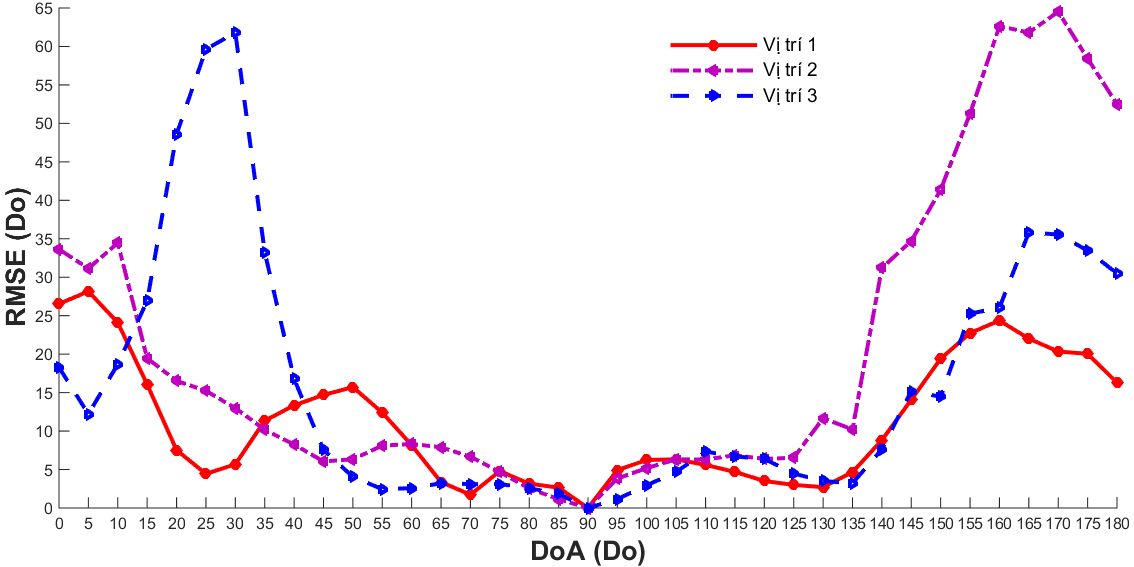
\includegraphics[width=1\linewidth]{figures/dvbt_1.png}
	\caption{RMSE: DOA ở từng vị trí thực nghiệm}
	\label{fig:dvbt_1}
\end{figure}

Từ kết quả RMSE thu được, có thể nhận thấy khoảng góc từ 60$^{\circ}$ đến 135$^{\circ}$ vẫn cho sai số thấp tương đương nhau ở cả 3 vị trí. Ở các góc ngoài khoảng trên, kết quả rất dễ bị ảnh hưởng bởi nhiễu đa đường, gây ra sai số nhảy vọt ở một số khoảng góc có nhiều vật cản.

Kết luận hệ ước lượng hướng sóng đến, vẫn hoạt động ở các điều kiện kênh truyền khác nhau.

\textbf{- Kết quả ước lượng với dữ liệu khác nhau}

Tuy theo lý thuyết, thuật toán MUSIC áp dụng cho mô hình tín hiệu băng hẹp, nhưng trong khóa luận này, sẽ mở rộng thêm và sử dụng tín hiệu băng rộng cho hệ DOA sử dụng thuật toán MUSIC.

Tín hiệu băng rộng được sử dụng là DVB-T, tín hiệu chuẩn thu truyền hình số mặt đất tiêu chuẩn ở Việt Nam. Việc điều chế, thông số, phổ DVB-T trên GNU Radio như sau: 

DVB-T: Điều chế chuẩn DVB-T trên GNU Radio với file nguồn là file video nén ở chuẩn TS (Transport Stream). Flow-graph ở phụ lục hình \ref{fig:dvbt} truyền video ở băng thông 8 MHz, chòm sao QPSK, tốc độ mã 7/8, khoảng bảo vệ 1/32, tốc độ lấy mẫu 10 MHz, tần số 923 MHz. Chi tiết hơn về việc sử dụng BladeRF truyền nhận DVB-T có tại \cite{BogdanDIA2015}.

Phổ tín hiệu DVB-T được truyền, và thu lại như hình \ref{fig:spectrum}, nhận thấy do sử dụng OFDM nên phổ của DVB-T bị trải đều trên dải tần số, dẫn đến SNR ở mức 37,5 dB so với trên 70 dB của NBFM.

\begin{figure} [!h]
	\centering
	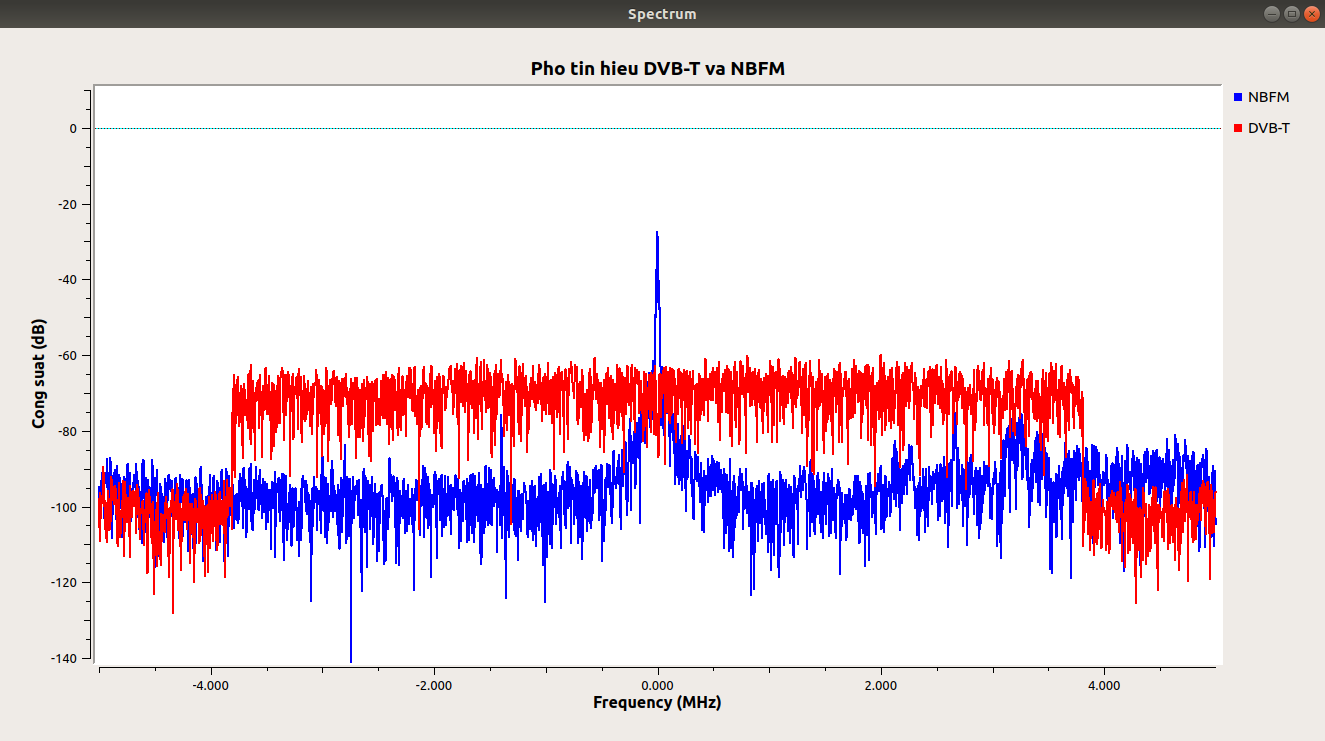
\includegraphics[width=1\linewidth]{figures/spectrum2.png}
	\caption{Phổ tín hiệu DVB-T và NBFM thu được}
	\label{fig:spectrum}
\end{figure}

Qua mô phỏng BladeRF trên GNU Radio, kết quả đồng bộ từ tín hiệu DVB-T thu được như bảng \ref{tab:kqdvbt}. Với tính tương quan thấp hơn của NBFM, kết quả ước lượng sai số phần cứng BladeRF từ tín hiệu DVB-T là hoàn toàn khớp với các thông số mô phỏng.
\begin{table}[!h]
	\caption{Kết quả mô phỏng đồng bộ bằng tín hiệu DVB-T}
	\centering
	\begin{tabular}{|l|l|l|cc|} 
		\hline
		\rowcolor[rgb]{1,0.91,0.906} \multicolumn{1}{|c|}{ \textbf{Loại tín hiệu} } & \multicolumn{1}{c|}{\textbf{Độ trễ (mẫu)} } & \multicolumn{1}{c|}{\textbf{Độ lệch pha (rad)} } & \multicolumn{2}{c|}{\textbf{Vector giá trị riêng} }  \\ 
		\hline
		\multirow{2}{*}{DVB-T}                                                      & \multirow{2}{*}{1000}                       & \multirow{2}{*}{0,78539}                         & 1,4544877e-11 & 0                                    \\
		&                                             &                                                  & 0             & 9,0942479e-04                        \\
		\hline
	\end{tabular}
\label{tab:kqdvbt}
\end{table}

Tuy nhiên qua thực nghiệm sử dụng tín hiệu băng rộng DVB-T cho đồng bộ và xác định hướng sóng đến, nhận thấy nếu thu toàn bộ 8 MHz băng thông của DVB-T sử dụng cho đồng bộ hệ BladeRF thì không thể thu được kết quả như mô phỏng. Vì vậy thay vì sử dụng toàn bộ dải băng rộng của tín hiệu DVB-T, tác giả khóa luận chỉ thu một phần của phổ DVB-T là 2 MHz, sau đó sử dụng thêm bộ lọc thông thấp 5 kHz như NBFM để lấy một phần nhỏ của tín hiệu DVB-T ban đầu, điều này khiến việc giải điều chế tín hiệu đồng thời như NBFM là không thể, tuy nhiên lại cho kết quả tốt khi xác định hướng sóng đến.

%Quay ngược lại mô phỏng việc sử dụng băng thông bộ thu chỉ 2 MHz và bộ lọc 5 kHz cho tín hiệu DVB-T, kết quả đồng bộ vẫn khớp với các thông số ban đầu đưa vào.
\newpage
Kết quả thực nghiệm trên hình \ref{fig:dvbt_3} khi thực nghiệm DOA tại một vị trí chỉ thay đổi tín hiệu bên phát, cho thấy dù ở khoảng 135$^{\circ}$ đến 180$^{\circ}$ sai số của DVB-T là nhỏ hơn NBFM nhưng nhìn chung thì trong khoảng góc quan trọng nhất là xung quanh 90$^{\circ}$ và hình dạng của đồ thị sai số của hai loại tín hiệu này vẫn là giống nhau và giữ được hình dạng như CRB.
\begin{figure} [!h]
	\centering
	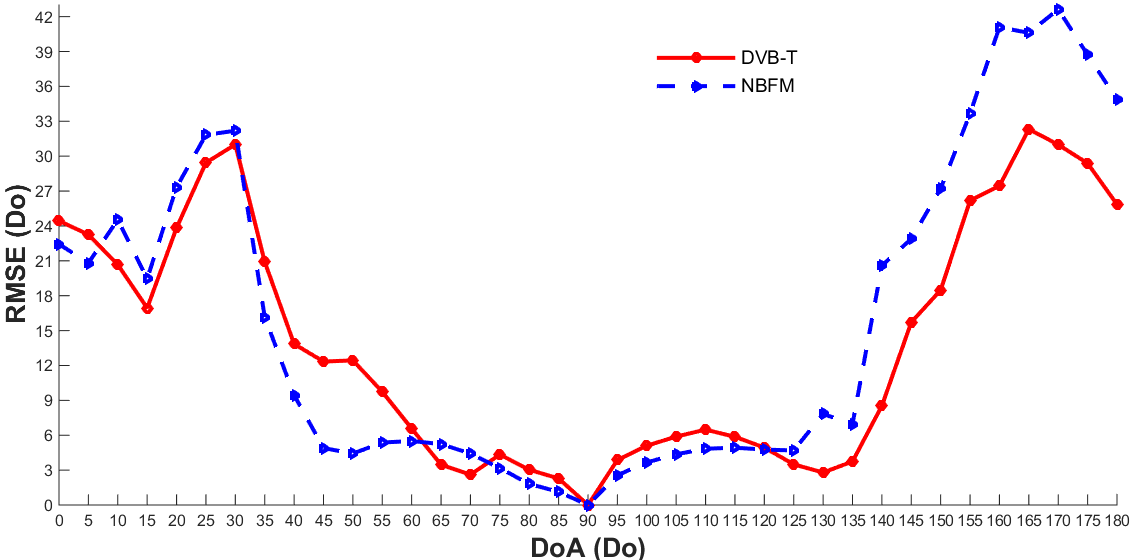
\includegraphics[width=1\linewidth]{figures/dvbt_3.png}
	\caption{RMSE: DOA với tín hiệu NBFM và DVB-T}
	\label{fig:dvbt_3}
\end{figure}

Kết luận lại, sử dụng tín hiệu băng rộng cho hệ DOA sử dụng thuật toán MUSIC hoàn toàn khả thi, kết quả thu được vẫn tốt giống như tín hiệu băng hẹp NBFM, tuy nhiên để tối ưu hơn hệ thống và tận dụng hết ưu thế của điều chế OFDM trong tín hiệu DVB-T thì tác giả cần phải tiếp tục nghiên cứu và phát triển thêm.
%Trong hình \ref{fig:dvbt_1} là kết quả sai số trung bình của hệ đặt DOA khi ở các vị trí khác nhau trong phòng, có thể nhận thấy, ở cả 3 vị trí thực nghiệm, khoảng góc từ 60$^{\circ}$ cho đến 140$^{\circ}$ đều cho sai số nhỏ dưới 6$^{\circ}$, đặc biệt ở các góc gần góc đồng bộ (90$^{\circ}$), sai số giảm xuống dưới 2$^{\circ}$. Điều này khớp với lý thuyết của hệ anten ULA, khi sai số sẽ tăng dần ở 2 biên của phổ công suất.

%Tuy nhiên, cũng dễ dàng nhận thấy, sai số tăng dần ở 2 biên không đều như lý thuyết mà có khoảng tăng vọt như: 35$^{\circ}$ đến 60$^{\circ}$ ở vị trí 1; 135$^{\circ}$ đến 160$^{\circ}$ ở vị trí 2; 15 đến 40 ở vị trí 3. Những sai số này được tạo ra bởi nhiễu đa đường, do anten VERT2450 được sử dụng là anten không định hướng, vì vậy ở các vị trí xuất hiện vật cản, nhiễu đa đường sinh ra làm tăng sự tương quan của 2 tín hiệu thu, và do thuật toán MUSIC yêu cầu tín hiệu thu không tương quan với nhau, kết quả thu được sẽ bị ảnh hưởng rất nhiều.
%\begin{figure} [!h]
%	\centering
%	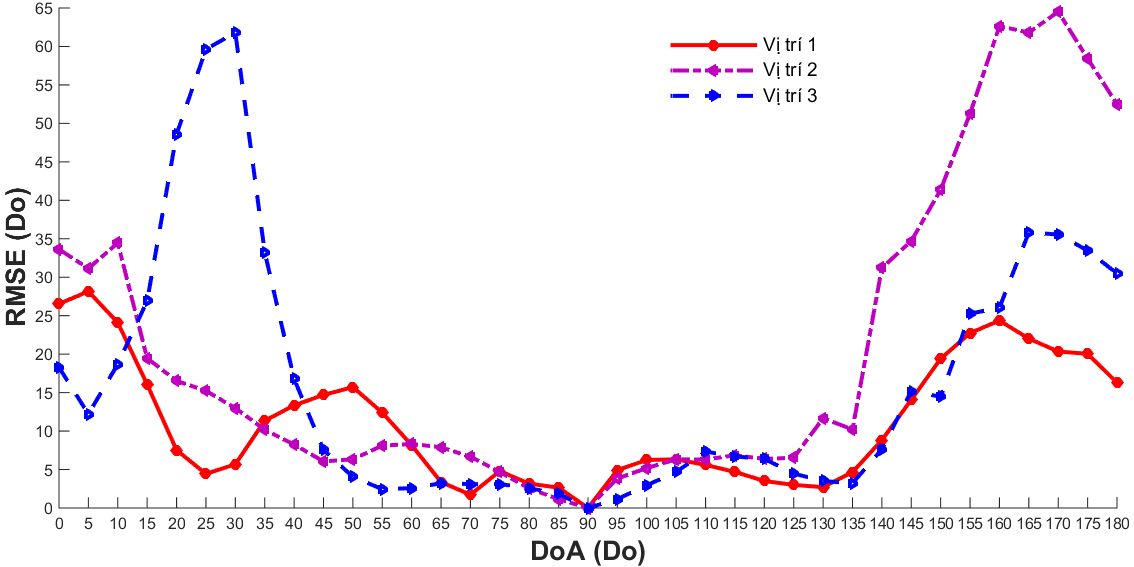
\includegraphics[width=1\linewidth]{figures/dvbt_1.png}
%	\caption{RMSE: DOA ở từng vị trí thực nghiệm}
%	\label{fig:dvbt_1}
%\end{figure}

%Ngoài sai số thay đổi do vị trí hệ thay đổi, tín hiệu được sử dụng để đồng bộ hệ DOA và tín hiệu phát để xác định hướng sóng đến cũng ảnh hưởng tới kết quả đầu ra. Kết quả trên hình \ref{fig:dvbt_3} cho thấy, có sự giống nhau về sai số ở những góc xung quanh 90$^{\circ}$, nhưng với các góc ở xa, tín hiệu DVB-T lại cho kết quả tốt hơn.

%NOTE: Trong thực nghiệm, theo em đo thì nếu đồng bộ bằng FM rồi chuyển sang DOA bằng loại tín hiệu khác, kqua sẽ dễ bị sai hơn. Còn DVB-T 64 QAM thì tương quan n thấp rồi, nên đồng bộ xong chuyển sang tín hiệu khác vẫn oke ạ.
%\begin{figure} [!h]
%	\centering
%	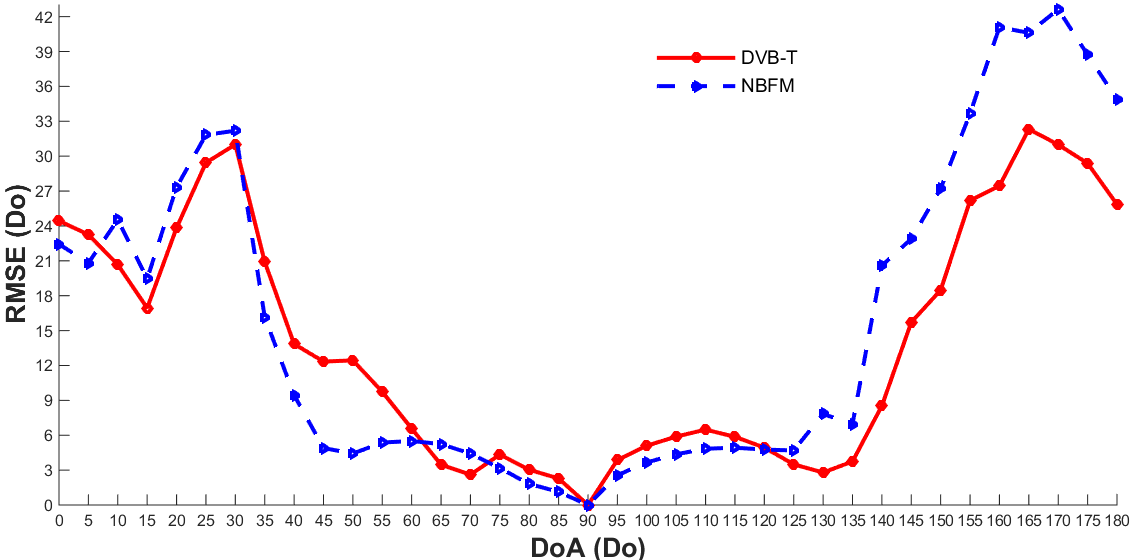
\includegraphics[width=1\linewidth]{figures/dvbt_3.png}
%	\caption{RMSE: DOA với tín hiệu NBFM và DVB-T}
%	\label{fig:dvbt_3}
%\end{figure}

%Tổng hợp lại, hình \ref{fig:kqdoa} là kết quả trung bình của toàn bộ quá trình thực nghiệm với hệ DOA trên BladeRF, có thể thấy hệ giảm độ chính xác đáng kể khi góc tới ở ngoài khoảng 40$^{\circ}$ đến 140$^{\circ}$, do nhiễu đa đường, hay độ phân giải của mảng thấp do chỉ sử dụng 2 phần tử anten thu và tính chất của mảng anten ULA.
%\begin{figure} [!h]
%	\centering
%	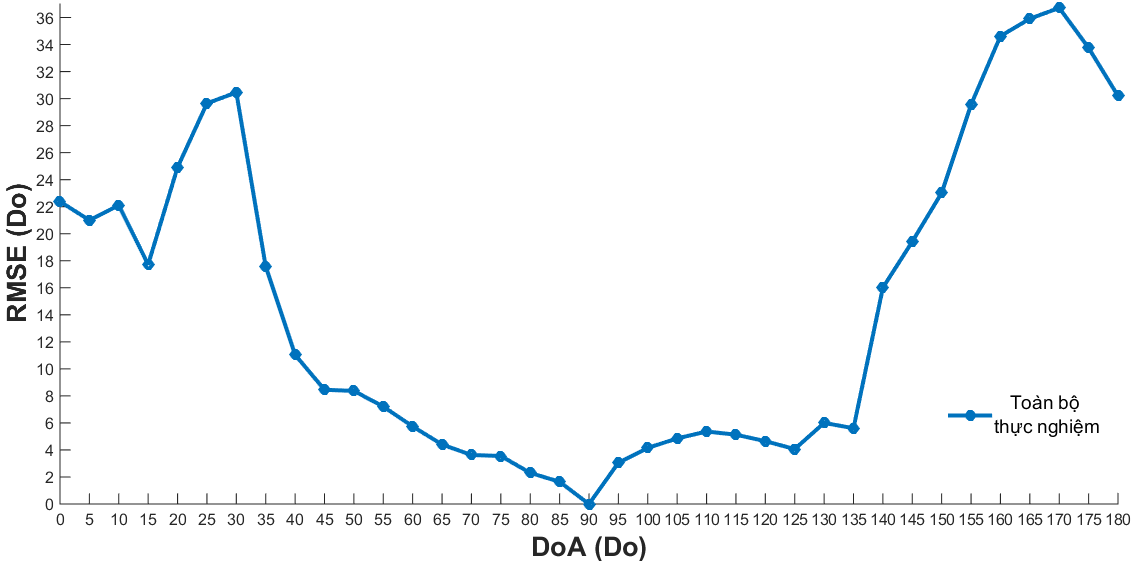
\includegraphics[width=1\linewidth]{figures/dvbt_2.png}
%	\caption{RMSE: DOA toàn bộ quá trình thực nghiệm}
%	\label{fig:kqdoa}
%\end{figure}
%
%\section{So sánh, đánh giá kết quả mô phỏng và kết quả thực nghiệm}

%So sánh với kết quả mô phỏng trên hình \ref{fig:kqsimu}, nhận thấy kết quả chung là ước lượng DOA cho sai số thấp ở các góc gần 90$^{\circ}$ tức góc căn chỉnh pha ban đầu, và càng ra xa về phía 2 biên sai số càng tăng nhanh. Tín hiệu chuẩn DVB-T có kết quả so sánh giữa hình \ref{fig:dvbt_3} và \ref{fig:kqsimu} khá khớp nhau về sai số ước lượng hướng sóng tới, tuy nhiên ở 2 biên, sai số tăng lên cao hơn so với mô phỏng.

%Không giống như sự chính xác ở kết quả mô phỏng, tín hiệu NBFM lại cho sai số gần như tương đồng với DVB-T mà không vượt trội như trên kết quả hình \ref{fig:kqsimu}, phần lớn sai số này phụ thuộc vào vị trí đặt hệ DOA, hay nguyên nhân chính là nhiễu đa đường, vì vậy có thể nhận xét, vị trí đặt hệ thu hay nhiễu đa đường là nguyên nhân chính khiến kết quả thực nghiệm sai số lớn hơn kết quả mô phỏng được.

%Và tổng hợp lại kết quả cuối cùng ở hình \ref{fig:kqdoa} so với CRB hình \ref{fig:RMSE} thì rõ ràng về dạng phổ thì có sự tương đồng, nhưng sai số là lớn hơn rất nhiều so với điều kiện lý tưởng trong giả thiết.